\section{Evaluation}

This section presents an in-depth empirical analysis of the design discussed in
Section~\ref{design-section}. To this end, we assess the scalability and
efficiency of the solution using multiple criteria.
%
First, an evaluation of the \textit{strong scaling} behavior of the distributed
algorithm is presented.
%
Second, the \textit{weak scaling} of the solution is assessed with respect to increasing
numbers of targeted latent communities.
%
Next, the effects of \textit{pipelining the computation} and varying the number of latent communities on the system's
performance is analyzed.
%
Further, we evaluate the efficiency and overhead associated with \textit{network
communication} between cluster nodes.
%
Finally, we \textit{contrast} the effectiveness of scaling the computation horizontally
and vertically.

Empirical results were obtained by performing experiments on the VU and
Leiden University
DAS5 clusters which consist of 68 and 24 compute nodes respectively. Each
compute node is equipped with a dual 8-core Intel Xeon E5-2630v3 CPU clocked
at 2.40GHz, 64GB of memory and 8TB of storage. Moreover, the compute nodes of
each site are interconnected by
FDR~InfiniBand. The MPI implementation used is MVAPICH2, which is optimally
tuned for Infiniband~\cite{mvapich}. All of the experiments reported in this section utilized
publicly available graphs from the Stanford Large Network Dataset
Collection~(SNAP) \cite{snapnets}. Table~\ref{tab-datasets} lists the
collection of data sets used.

%################################################
\subsection{Weak Scaling}

\begin{figure}[t] % [htbp]
  \centering
  
\epsfig{file=plots/sweep-over-K-proportional-np.eps, width=0.48\textwidth}
  \caption{Average execution time per algorithm iteration when varying
  the number of latent communities proportionally to the number of compute
  nodes.}
  \label{fig-weak-scaling}
\end{figure}

A study of a system's weak scaling aids in the assessment of the communication
and synchronization overheads associated with the management of large clusters.
Similarly, it can expose complex issues that hinder performance at scale such
as load imbalance. To fairly evaluate the algorithm's weak scaling behavior we
conducted several executions varying the cluster size and the number of latent
communities proportionally. The number of communities is 192 times the number
of worker nodes in all runs.
This methodology ensures that each compute node
performs an approximately constant amount of computational work across all
configurations. However, the number and size of messages exchanged between the
nodes would vary significantly. Figure~\ref{fig-weak-scaling} presents the
average execution
time per algorithm iteration across different cluster sizes.
This figure shows that the system's overall
overhead is minimal. Additionally, the experimental results show that the
implementation is capable of achieving good speedups provided the input problem
is large enough for the given cluster size.

%################################################
\subsection{Strong Scaling}

\begin{figure}[t] % [htb]
  \centering
  \epsfig{file=plots/sweep-over-np-fixed-K.eps, width=0.48\textwidth}
  \caption{(a) Execution time of 2048 algorithm iterations for the
  same problem size (com-Friendster, K=1024, M=16384 n=32) across different
  cluster sizes. (b) Speedup achieved for same experiments in (a) with respect to
  8 nodes}
  \label{fig-strong-scaling}
\end{figure}

In order to evaluate the horizontal scalability of the distributed
implementation we tested the system's performance across different cluster
sizes while holding the problem size constant. For this study, we used the
com-Friendster graph as it contains the largest number of vertices and edges.
%
Figure~\ref{fig-strong-scaling}-a presents the execution time of 2048 algorithm
iterations across multiple cluster sizes. The x-axis starts from 8 worker nodes
as the data set is too large to fit into the collective memory of a smaller
cluster.
%
As shown in the figure, the execution
time steadily decreases by increasing the cluster size.
A deeper analysis of the individual execution phases of the algorithm provides
insights into the scalability of its building blocks.
%
In addition to the total execution time, Figure~\ref{fig-strong-scaling}-a
presents the cumulative time spent in individual computational phases across
iterations. Moreover, Figure~\ref{fig-strong-scaling}-b presents the speedup
achieved for the same experiments reported in
Figure~\ref{fig-strong-scaling}-a. As is clearly shown, the dominant phase of
the execution is \textit{update\_phi\_pi}.
The reported total time for each cluster size is significantly less than the
sum of the execution times of the individual phases. This is due to the
overlapping execution of the two most expensive phases, namely,
\textit{update\_phi\_pi} and
mini-batch deployment. Both of these phases initially gain significant speedup with the
addition of compute nodes. However, the speedup curve gradually slows down for
larger cluster sizes as the work granularity of each worker node decreases,
limiting their resource utilization.
%
The time spent in \textit{update\_beta\_theta} remains relatively constant across cluster sizes
as it performs an insignificant amount of work compared to the synchronization
overhead of a collective MPI reduction operation contained within it.

%################################################
\subsection{Pipeline efficiency}
\label{eval-pipeline}

As discussed in Section~\ref{design-section}, we implemented pipeline
parallelism at
two places in the algorithm. The first is an inter-process pipeline that
overlaps drawing of the mini-batch at the master's with \textit{update\_phi}
at the workers. The second pipeline overlaps loading of $\pi$ with the
computation within \textit{update\_pi} within each worker.

\begin{table}[t] % [htbp]
  \centering
  \begin{tabular}{l d{5.1} d{5.1}}
    \textbf{Iteration (sub)stages}  & \multicolumn{1}{c}{non-pipelined}
                                          & \multicolumn{1}{c}{pipelined} \\
    \hline
    draw/deploy mini-batch     &  45.6  &  26.2 \\
    load $\pi$                 & 205    & 209 \\
    update $\phi$              &  74    &  74 \\
    \hline
    total                      & 331    & 241 \\
    \hline
  \end{tabular}
  \caption{Stages that profit from the two pipelining optimizations.
  com-Friendster on 65
  compute nodes, with 12K communities. Times in ms per iteration.}
  \label{table-pipeline}
\end{table}

Table~\ref{table-pipeline} shows a breakdown of the (sub)stages that are
overlapped by both pipelining optimizations. The left-hand column has
all pipelining disabled, the right-hand
column has pipelining enabled. Within \textit{update\_phi},
loading $\pi$ from the DKV store is dominant.
The pipelining optimization significantly overlaps loading $\pi$ both with generation and
deployment of the mini-batch, and with the calculation of \textit{update\_phi}.

\begin{figure}[t] % [htb]
  \centering
  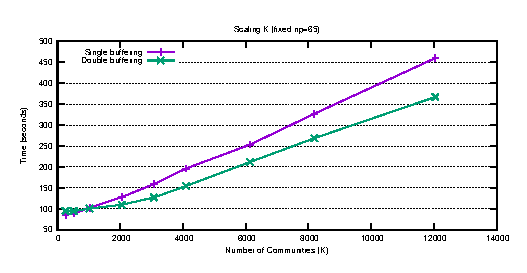
\epsfig{file=plots/sweep-over-K-fixed-np.eps, width=\columnwidth}
  \caption{Performance effect of varying the number of communities on the
    algorithm's execution time on 64 nodes when disabling or enabling both
    pipelining optimizations.}
  \label{fig-pipeline}
\end{figure}

Figure~\ref{fig-pipeline} presents the execution time of 1024 algorithm
iterations on a 64-node cluster with the pipelines enabled and disabled.
Naturally, increasing the number of communities causes a proportional increase
in execution time. However, when pipelining is enabled, some of the
incurred network latency is hidden by overlapping it with computation.
Moreover, since both computation time and network latency increase with larger
$K$, the benefit of pipelining increases. This can be observed through the
widening gap between both lines depicted in Figure~\ref{fig-pipeline}.
Large cluster
configurations exhibit higher bandwidth demands and are more sensitive
to network latency:
given that $\pi$ accesses are random, a node in a cluster of size $C$ must
fetch $(C-1)/C$ of all read requests over the network.

%################################################
\subsection{Horizontal vs. Vertical Scalability}
\begin{figure}[t] % [htb]
  \centering
  
\epsfig{file=plots/hpc-cloud.eps, width=0.48\textwidth}
  \caption{Performance comparison between the distributed implementation
  running on DAS5 and the multi-threaded solution on machine with 40 cores and
  1TB of RAM.}
  \label{fig-scale-up}
\end{figure}
One of the main drawbacks of designing a distributed solution for a given
algorithm is the inherent complexity of communication and synchronization. A
considerably simpler approach would be developing a multi-threaded version and
running it on a machine with abundant memory and CPU cores. In such a context,
access to all of the algorithm's state would be an order of magnitude faster
than RDMA. Additionally, the overhead associated with synchronizing threads is
negligible compared to using MPI primitives. To evaluate the efficacy of both
approaches we utilized SURFsara's HPC Cloud system to instantiate a virtual
machine with 40 Intel Xeon E7-4850 cores clocked at 2.00GHz cores and 1TB of
memory. The physical machine underlying
the HPC Cloud system contains 40~CPU cores and does not oversubscribe
resources. Therefore, by provisioning all 40~cores we ensured that there is no
resource contention from other users of the system. Figure~\ref{fig-scale-up}
reports the execution time per algorithm iteration for two experimental setups.
%
First, Figure~\ref{fig-scale-up}-a shows the performance of executing the
algorithm on the HPC Cloud
system with 40 and 16 cores compared to a single DAS5 node with 16~cores. This
test uses the com-DBLP data set to enable the use of a large number of
communities without running out of memory. It is clear from the results that
the performance can benefit from the additional cores provided by HPC Cloud system.
%
Further, Figure~\ref{fig-scale-up}-b tests the performance of the HPC Cloud
system compared to 64 nodes of the DAS5
cluster using the com-Friendster data set. Clearly, the parallel and
distributed implementation vastly
outperforms the single-node multi-threaded solution. Moreover, the trajectory
of both curves shows a widening gap between them suggesting that the relative
performance difference will increase for larger $K$.
%
In conclusion, the overhead of network communication in the distributed version
is more than compensated by the increasing compute power compared to
a single-node implementation.

%################################################
\subsection{Cluster Communication Efficiency}

\begin{figure}[b] % [htbp]
  \centering
  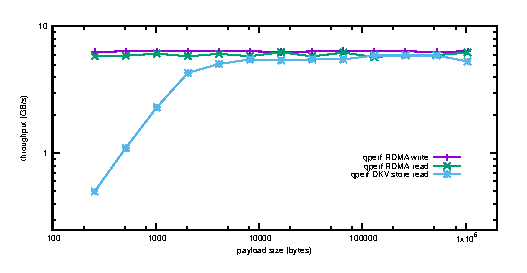
\epsfig{file=plots/qperf.eps, width=0.5\textwidth}
  \caption{Performance of DKV store compared to qperf and MPI roundtrip.}
  \label{fig-qperf}
\end{figure}

\begin{figure*}[htbp] % [htb]
  \centering
  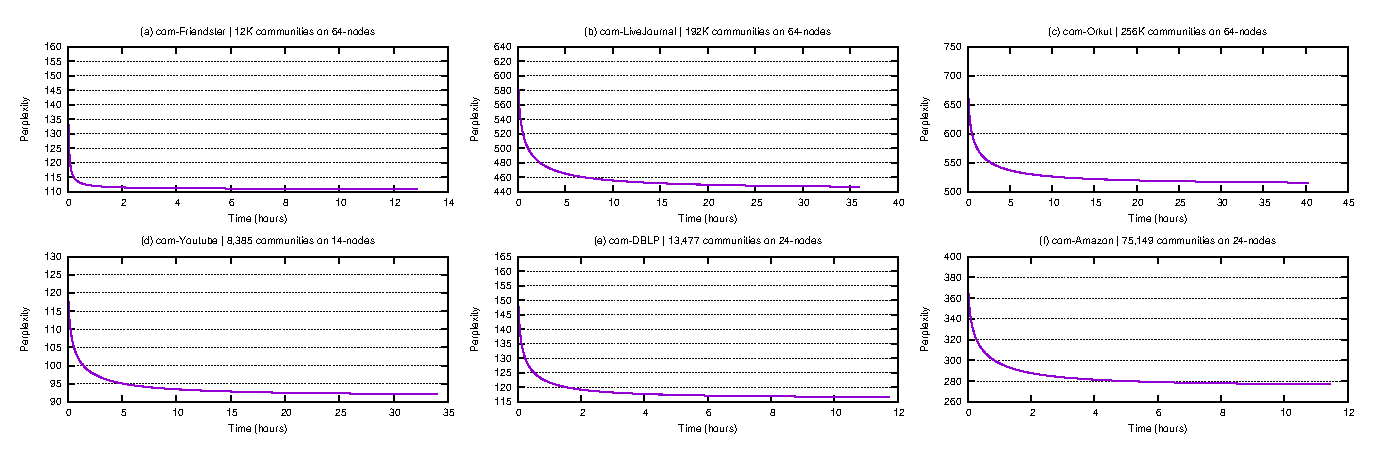
\epsfig{file=plots/ppx.eps, width=\textwidth}
  \caption{Convergence time of 6 different data sets.}
  \label{fig-ppx}
\end{figure*}

Since the distributed algorithm is data-intensive, a key aspect in improving
its performance is to maximize the utility of the network resources.
In figure~\ref{fig-qperf}, we provide maximum bandwidth numbers for
read operations between one server and one client for a range of payload sizes,
and compare these to the bandwidth achieved by an MPI roundtrip test,
and by \textit{qperf}~\cite{qperf-mellanox} which reports
the best achievable performance for Infiniband. We present \textit{qperf}
bandwidth for both RDMA read and RDMA write operations; these are nearly
identical, which corroborates the results from the Herd project for payloads
upwards from 256B.
The MVAPICH2 implementation
is highly optimized for Infiniband. It requires an interaction between
the server network card and the server host, which increases the latency and
thus lowers the bandwidth
significantly. This is ample justification for using a low-level RDMA
implementation for the DKV store.
The bandwidth achieved by our DKV store falls short
of the \textit{qperf} performance for packets less than 4KB; this is attributed
to additional per-request overhead for the DKV store. For the largest packet
size, the DKV store performance is hampered by the fact that its values
are spread over a larger memory area, whereas \textit{qperf} and MPI always reads
from the same memory locations. For packets between 8KB and 512KB, our DKV
achieves performance very close to \textit{qperf}.

%################################################
\subsection{Convergence of Large Datasets}

The previous sections focused on the computational performance of the
distributed implementation. However, the algorithm's throughput does not
necessarily indicate how fast it can converge to a solution. More specifically, it
remains unclear how many iterations are needed for the algorithm to reach a
stable state and terminate. Therefore, we now shift our focus to the
convergence time to assess the system's utility. Figure~\ref{fig-ppx} presents
the convergence time of the data sets listed in Table~\ref{tab-datasets}.
%
The results in sub-figures a, b and c were obtained by using 65 compute nodes
of DAS5. In Figure~\ref{fig-ppx}-a, the number of communities was set to 12K
which fully occupied the aggregate memory resources of all 64 worker nodes since
com-Friendster has roughly 65 million vertices. In this case, the algorithm
reached a stable state after 3-4 hours. Next, Figures~\ref{fig-ppx}-b and
\ref{fig-ppx}-c present the convergence of com-LiveJournal and com-Orkut
respectively. As the number of vertices in these data sets is an order of
magnitude smaller than com-Friendster, we could use a larger number of
communities to fill up the collective memory. Naturally, the convergence time was extended as the complexity of
the algorithm increases dramatically with larger K. However, the system was
capable of reporting results for both in around 40 hours.
%
Figures~\ref{fig-ppx}-d, \ref{fig-ppx}-e and \ref{fig-ppx}-f were all
configured to use the number of ground-truth communities associated with
their respective data sets, com-Youtube, com-DBLP and com-Amazon. Since this
yields a much smaller storage requirement,
these experiments were conducted on 14, 24 and 24 cluster nodes respectively.

The results reported in Figure~\ref{fig-ppx} verify that the distributed
implementation of the algorithm is capable of detecting overlapping communities
within real graphs in reasonable time given the available compute resources.
The time required to reach convergence may vary depending on a graph's properties and
the targeted number of communities. To the best of our knowledge, the data sets
used in this study are the largest publicly available organic graphs.

